\section{Project Implementation}

\subsection{Overview of Project Modules}
\textbf{Users:-}\\
First user open browser and enter url
\begin{itemize}
	\item  Registration.
	\item Login.
	\item Request speech to text or request.
	\item Stope word elimination wich are not excelent for analysis 
	\item Classify Request type.
	\item find out solution
	\item Send request to department.
	
\end{itemize}
\textbf{Postprocessing:-}\\
 means server system it include,
\begin{itemize}
	\item User request accept 
	\item Word elimanation stoping.
	\item display final output.
	\item Request send succesfully .


\end{itemize}

\subsection{Tools and Technologies Used }

\begin{itemize}
	\item \textbf{JAVA:}\\
	Java is one of the most popular and widely used programming language and platform. A platform is an environment that helps to develop and run programs written in any programming language.\\
	Java is fast, reliable and secure. From desktop to web applications, scientific supercomputers to gaming consoles, cell phones to the Internet, Java is used in every nook and corner.\\
	Java is a programming language and computing platform first released by Sun Microsystems in 1995. There are lots of applications and websites that will not work unless you have Java installed, and more are created every day. Java is fast, secure, and reliable. From laptops to datacenters, game consoles to scientific supercomputers, cell phones to the Internet, Java is everywhere! \\
	Java is a general-purpose, concurrent, object-oriented, class-based, and the runtime environment(JRE) which consists of JVM which is the cornerstone of the Java platform. This blog on What is Java will clear all your doubts about why to learn java, features and how it works.\\
	
	\item \textbf{XAMPP:}\\
	XAMPP stands for Cross-Platform (X), Apache (A), MySQL (M), PHP (P) and Perl (P). It is a simple, lightweight Apache distribution that makes it extremely easy for developers to create a local web server for testing purposes. Everything you need to set up a web server – server application (Apache), database (MySQL), and scripting language (PHP) – is included in a simple extractable file. XAMPP is also cross-platform, which means it works equally well on Linux, Mac and Windows. Since most actual web server deployments use the same components as XAMPP, it makes transitioning from a local test server to a live server is extremely easy as well. Web development using XAMPP is especially beginner friendly.\\
	
	\item \textbf{JDK:}\\ The Java Development Kit (JDK) is an implementation of either one of the Java Platform, Standard Edition, Java Platform, Enterprise Edition, or Java Platform, Micro Edition platforms released by Oracle Corporation in the form of a binary product aimed at Java developers on Solaris, Linux, macOS or Windows. The JDK includes a private JVM and a few other resources to finish the development of a Java Application. Since the introduction of the Java platform, it has been by far the most widely used Software Development Kit (SDK).[citation needed] On 17 November 2006, Sun announced that they would release it under the GNU General Public License (GPL), thus making it free software. This happened in large part on 8 May 2007, when Sun contributed the source code to the OpenJDK.\\
	
	\item \textbf{Apache:}\\ Apache is the actual web server application that processes and delivers web content to a computer. Apache is the most popular web server online, powering nearly 54 percent of all websites.\\
	
	\item \textbf{MySQL:}\\ Every web application, howsoever simple or complicated, requires a database for storing collected data. MySQL, which is open source, is the world’s most popular database management system. It powers everything from hobbyist websites to professional platforms like WordPress. You can learn how to master PHP with this free MySQL database for beginners course.\\
\end{itemize}
%\begin{figure}[h!]
%\centering
%\fbox{\includegraphics[scale = .375]{./querysug}}
%\caption[Graph construction for query suggestion]{Graph construction for query suggestion. (a) Query-URL bipartite graph. (b) Converted query-URL bipartite graph.}
%\label{fig:querysug}
%\end{figure}

\subsection{Algorithmic Details}
\paragraph{}In our project we use TF*IDF algorithm is an information retrieval technique that weighs a term’s frequency (TF) and its inverse document frequency (IDF). Each word or term that occurs in the text has its respective TF and IDF score.\\
The product of the TF and IDF scores of a term is called the TF*IDF weight of that term. Put simply, the higher the TF*IDF score (weight), the rarer the term is in a given document and vice versa.\\
The TF*IDF algorithm is used to weigh a keyword in any content and assign importance to that keyword based on the number of times it appears in the document. More importantly, it checks how relevant the keyword is throughout the web, which is referred to as corpus.\\

Gather words. Write your content. Run a TF*IDF report for your words and get their weights. The higher the numerical weight value, the rarer the term. The smaller the weight, the more common the term. Compare all the terms with high TF*IDF weights with respect to their search volumes on the web. Select those with higher search volumes and lower competition. Work smart.\\

A good rule of thumb is, the more your content “makes sense” to the user, the more weight it is assigned by the search engine. With words having a high TF*IDF weight in your content, your content will always be among the top search results, so you can:\\

stop worrying about using the stop-words.\\
successfully hunt words with higher search volumes and lower competition\\
be sure to have words that make your content unique and relevant to the user, etc.\\




\subsubsection{Algorithm 1: }
TF*IDF is an information retrieval technique that weighs a term's frequency (TF) and its inverse document frequency (IDF). Each word or term that occurs in the text has its respective TF and IDF score. TF*IDF is used by search engines to better understand the content that is undervalued. \\
Step 1 :Tokenize the sentences. \\
Step 2 :Create the Frequency matrix of the words in each sentence.\\
Step 3: Calculate TermFrequency and generate a matrix. \\
Step 4: Creating a table for documents per words. 
Step 5 : Calculate IDF and generate a matrix.\\
Step 6: Calculate TF-IDF and generate a matrix.\\
Step 7: Score the sentences.\\
Step 8: Find the threshold.\\
\subsubsection{Algorithm 2: K-Means }
K-means is a centroid-based algorithm, or a distance-based algorithm, where we calculate the distances to assign a point to a cluster. In K-Means, each cluster is associated with a centroid.
\begin{figure}[!h]
	\centering
	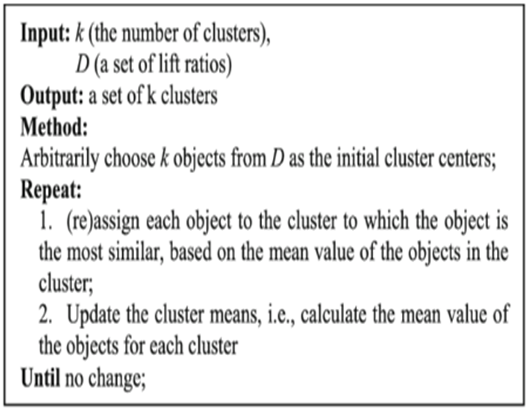
\includegraphics[width = \textwidth]{./algo1}
	
\end{figure}

